\documentclass{standalone}
\usepackage{hsbcommon}
\makeatletter\AtBeginDocument{\@buildstepset{0,1,2,3,4,5,6}}\makeatother
\begin{document}
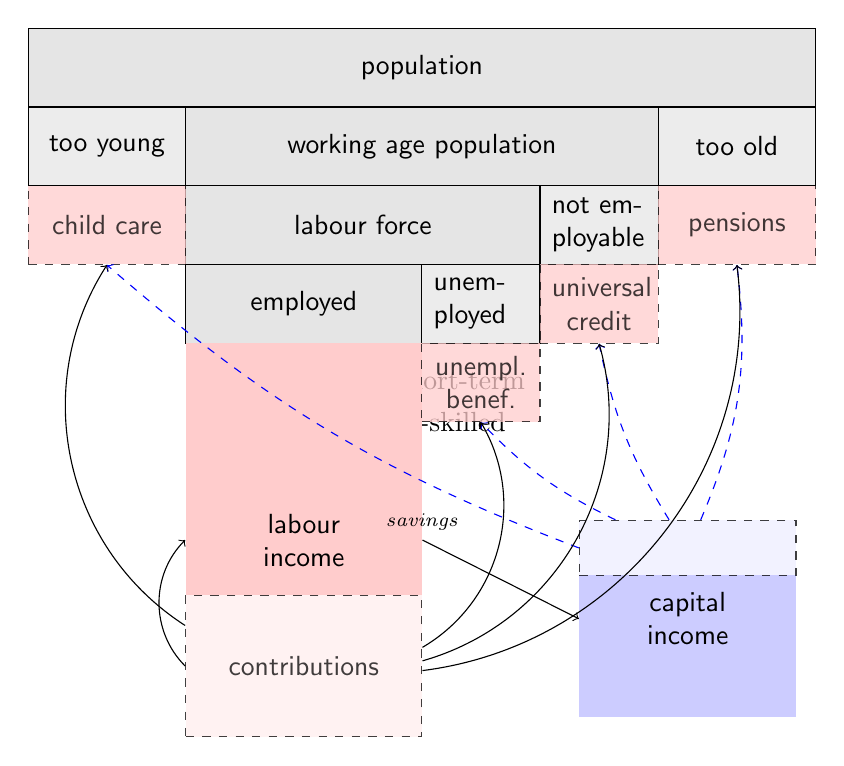
\begin{tikzpicture}
    \tikzset{
        myboxed/.style={
                draw,
                minimum height=1cm,
                anchor=west,
                fill=gray!20,
                align=center,
                font=\sffamily
            },
        mywages/.style={
                % draw,
                minimum height=1cm,
                anchor=west,
                fill=red!20,
                align=center,
                font=\sffamily       
        },        
        mygains/.style={
                % draw,
                minimum height=1cm,
                anchor=west,
                fill=blue!20,
                align=center,
                font=\sffamily       
        },
        mytransfer/.style={
                minimum height=1cm,
                anchor=west,
                fill=white,
                opacity=0.75,
                draw, 
                dashed,
                align=center,
                font=\sffamily       
        }, 
        mybenefit/.style={
                minimum height=1cm,
                anchor=west,
                fill=red!20,
                opacity=0.75,
                draw,dashed,  
                align=center,
                font=\sffamily       
        },
        unboxed/.style={
                minimum height=1cm,
                fill=gray!15,
                draw,
                anchor=west,
                font=\sffamily
            }
        }
    \node[myboxed,minimum width=10cm] at (0,0) {population};
    \node[myboxed,minimum width=6cm] at (2,-1) {working age population};
        \node[unboxed,minimum width=2cm] at (0,-1) {too young};
        % \node[unboxed,text width=2cm] at (0,-1.5) {in education};
        \node[unboxed,minimum width=2cm] at (8,-1) {too old};
    \node[myboxed,minimum width=4.5cm] at (2,-2) {labour force};
        \node[unboxed,minimum width=1.5cm,
        text width=1.2cm] at (6.5,-2) {not employable};
    \node[myboxed,minimum width=3cm] at (2,-3) {employed};
        \node[unboxed,minimum width=1.5cm,text width=1.2cm] at (5,-3) {un\-em\-ployed};

    \ifsteponly{1}{2,3,4}{
        \node[anchor=west, minimum width=5cm] at (2,-4) {long-term \& short-term};
        \node[anchor=west, minimum width=5cm] at (2,-4.5) {skilled \& non-skilled};
    }

    \ifstep{2}{
       \node[mywages,minimum width=3cm,text width=2cm, minimum height=5cm] (wages) at (2,-6) {labour income};
    }

    \ifstep{3}{
        \node[mybenefit,minimum width=2cm,text width=1.5cm] (childcare) at (0,-2) {child care};
    }
    \ifstep{3}{
        \node[mybenefit,minimum width=1.5cm,text width=1.2cm] (benefits) at (5,-4) {unempl. benef.};
    }
     \ifstep{3}{
        \node[mybenefit,minimum width=1.5cm,text width=1.2cm] (credit) at (6.5,-3) {universal credit};
    }
    \ifstep{3}{
        \node[mybenefit,minimum width=2cm,text width=1.5cm] (pensions) at (8,-2) {pensions};
    }

    \ifstep{5}{
       \node[mygains,minimum width=2.75cm,text width=1.5cm, minimum height=2.5cm] (gains) at (7,-7) {capital income};
    }

    \ifstep{6}{
        \node[mytransfer,minimum width=2.75cm,minimum height=0.7cm] (transfer2) at(7,-6.1) {} ;
        \draw[dashed,blue,->,bend right=15] (transfer2) to (pensions.south);
        \draw[dashed,blue,->,bend left=10] (transfer2) to (credit.south);
        \draw[dashed,blue,->,bend left=10] (transfer2) to (benefits.south);
        \draw[dashed,blue,->,bend left=10] (transfer2.west) to (childcare.south);
    }

    \ifstep{4}{
        \node[mytransfer,minimum width=3cm,minimum height=1.8cm] (transfer) at(2,-7.6) {contributions} ;
        \draw[->,bend right=45] (transfer) to (pensions.south);
        \draw[->,bend right=45] (transfer) to (credit.south);
        \draw[->,bend right=45] (transfer) to (benefits.south);
        \draw[->,bend left=45] (transfer) to (childcare.south);
    }

    \ifstep{6}{
        \draw[->,bend left=45] (transfer.west) to (wages.west);
    }
    \ifstep{7}{
        \draw[->] (wages.east) node[above]{\scriptsize \textit{savings}} to  (gains.west) ;
    }
    
    
\end{tikzpicture}
\end{document}